% Shared preamble for the multilayer-perceptron exercises.
% Each exercise is a standalone document: compile it from this directory.
\documentclass[11pt,a4paper]{article}

\usepackage[margin=2.35cm,top=1.85cm,bottom=2.15cm,headheight=22pt,headsep=9pt]{geometry}
\usepackage[T1]{fontenc}
\usepackage[utf8]{inputenc}
\usepackage[english]{babel}
\usepackage{lmodern}
\usepackage{textcomp}
\usepackage{microtype}
\usepackage{amsmath,amssymb,amsthm,mathtools}
\usepackage{booktabs}
\usepackage{array}
\usepackage{enumitem}
\usepackage{xcolor}
\usepackage{tikz}
\usetikzlibrary{arrows.meta,positioning,calc}
\usepackage{pgfplots}
\pgfplotsset{compat=1.17}
\usepackage[hypcap=false]{caption}
\usepackage{needspace}
\usepackage{titlesec}
\usepackage{fancyhdr}
\usepackage[hidelinks,unicode]{hyperref}

\setlength{\parindent}{1.15em}
\setlength{\parskip}{0pt}
\setlength{\abovedisplayskip}{7pt plus 2pt minus 2pt}
\setlength{\belowdisplayskip}{7pt plus 2pt minus 2pt}
\setlength{\abovedisplayshortskip}{4pt plus 2pt}
\setlength{\belowdisplayshortskip}{5pt plus 2pt}
\setlength{\emergencystretch}{2em}
\allowdisplaybreaks[1]

\definecolor{navy}{HTML}{1B365D}
\definecolor{ink}{HTML}{1C1917}
\definecolor{rulegold}{HTML}{8C6A32}
\definecolor{wash}{HTML}{F6F3EC}
\definecolor{accent}{HTML}{7A2E2E}

\pagestyle{fancy}
\fancyhf{}
\fancyhead[L]{\small\sffamily\color{navy}Universidad Pontificia Comillas}
\fancyhead[R]{\small\sffamily\color{navy}\exerciseshort}
\fancyfoot[C]{\small\color{ink!70}\thepage}
\renewcommand{\headrulewidth}{0.4pt}
\renewcommand{\headrule}{%
  \hbox to\headwidth{\color{rulegold}\leaders\hrule height \headrulewidth\hfill}%
}
\fancypagestyle{plain}{%
  \fancyhf{}%
  \fancyfoot[C]{\small\color{ink!70}\thepage}%
  \renewcommand{\headrulewidth}{0pt}%
}

\captionsetup{
  font={small},
  labelfont={sf,bf,color=navy},
  labelsep=period,
  skip=7pt
}

\titleformat{\section}
  {\Large\bfseries\sffamily\color{navy}}
  {\thesection}{0.55em}{}
  [\vspace{0.2em}{\color{navy}\titlerule[0.55pt]}]
\titleformat{\subsection}
  {\normalsize\bfseries\sffamily\color{navy}}
  {}{0pt}{}
  [\vspace{-0.15em}{\color{rulegold}\titlerule[0.4pt]}]
\titlespacing*{\section}{0pt}{1.15em}{0.55em}
\titlespacing*{\subsection}{0pt}{1.05em}{0.4em}

\theoremstyle{plain}
\newtheorem{lemma}{Lemma}
\newtheorem{proposition}{Proposition}
\theoremstyle{definition}
\newtheorem*{remark}{Remark}

\setlist[enumerate]{leftmargin=1.7em,itemsep=0.5em,topsep=0.35em,labelsep=0.5em}
\setlist[itemize]{leftmargin=1.35em,itemsep=0.25em,topsep=0.3em}

\newcommand{\exerciseshort}{Multilayer perceptrons}
\newcommand{\R}{\mathbb{R}}
\newcommand{\E}{\mathbb{E}}
\DeclareMathOperator{\Var}{Var}
\DeclareMathOperator{\relu}{ReLU}
\DeclarePairedDelimiter{\abs}{\lvert}{\rvert}
\DeclarePairedDelimiter{\norm}{\lVert}{\rVert}
\newcommand{\dd}{\mathrm{d}}
\newcommand{\T}{\mathsf{T}}

\tikzset{
  neuron/.style={
    circle, draw=navy, line width=0.65pt, minimum size=8.2mm,
    inner sep=0pt, font=\small, fill=white
  },
  ninput/.style={neuron, fill=navy!6},
  nhidden/.style={neuron, fill=navy!11},
  noutput/.style={neuron, fill=rulegold!18},
  ndead/.style={neuron, fill=ink!8, draw=ink!45, text=ink!55},
  nedge/.style={
    -{Stealth[length=1.65mm,width=1.35mm]},
    draw=ink!72, line width=0.45pt
  },
  ntag/.style={font=\scriptsize\sffamily, text=navy}
}

% #1 number, #2 running head, #3 display title, #4 introductory paragraph
\newcommand{\exercisefront}[4]{%
  \thispagestyle{plain}%
  \gdef\exerciseshort{Exercise #1\enspace\textperiodcentered\enspace #2}%
  \noindent{\sffamily\footnotesize\color{navy}%
    \MakeUppercase{Universidad Pontificia Comillas}}\par
  \vspace{0.15em}
  \noindent{\sffamily\footnotesize\color{ink!80}%
    Teaching collection of Eduardo C\'esar Garrido Merch\'an}\par
  \vspace{0.55em}
  \noindent{\sffamily\small\color{ink!75}%
    Multilayer perceptrons%
    \enspace\textcolor{rulegold}{\textperiodcentered}\enspace
    Exercise #1 of 3}\par
  \vspace{0.7em}
  \noindent{\sffamily\LARGE\bfseries\color{navy}#3\par}
  \vspace{0.35em}
  \noindent{\color{rulegold}\rule{\textwidth}{0.7pt}}\par
  \vspace{0.75em}
  \noindent #4\par
  \vspace{0.15em}
}

\newcommand{\solutionpart}[1]{%
  \Needspace{8\baselineskip}%
  \subsection*{Solution to (#1)}%
}

\hypersetup{
  pdfauthor={Eduardo C\'esar Garrido Merch\'an},
  pdfsubject={Graduate exercises on multilayer perceptrons}
}

\hypersetup{pdftitle={Exercise 2. Expressivity and universal approximation}}

\begin{document}

\exercisefront{2}{Expressivity}
  {Expressivity and universal approximation}
  {A multilayer perceptron with a ReLU activation computes a continuous piecewise-linear function. This exercise makes that description exact in one variable, uses it to represent a triangular bump and the Boolean XOR, and then compares a shallow network with a deep one on a family of increasingly oscillatory targets. The last question is the universal approximation theorem in one variable, together with the reason a polynomial activation falls outside it. No external theorem is required for the proofs; the multivariate statement is recorded, with its sources, only at the end.}

\section{Setup}

The rectified linear unit is \(\relu(t) = \max\{t, 0\}\). It is applied elementwise to vectors. A \emph{one-hidden-layer ReLU network} of width \(m\), with univariate input, is a function of the form
\begin{equation}
  g(x)
  =
  c + \sum_{i=1}^{m} v_i\,\relu(w_i x + b_i),
  \qquad
  c,v_i,w_i,b_i\in\R.
  \label{eq:shallow}
\end{equation}
A network with \(n\) hidden layers is the analogous alternation of affine maps and coordinatewise ReLUs, ending in a linear readout. Depth is measured by the number of hidden layers, so \eqref{eq:shallow} has one hidden layer regardless of \(m\).

Two target functions are fixed for the whole exercise. The triangular bump \(f:\R\to\R\) is
\begin{equation}
  f(x) =
  \begin{cases}
    0 & \text{if } x < 0,\\
    x & \text{if } 0 \le x < 1,\\
    2-x & \text{if } 1 \le x < 2,\\
    0 & \text{if } x \ge 2,
  \end{cases}
  \label{eq:bump}
\end{equation}
and the tent map \(s:[0,1]\to[0,1]\) is
\begin{equation}
  s(x) =
  \begin{cases}
    2x & \text{if } 0 \le x \le \tfrac12,\\
    2-2x & \text{if } \tfrac12 \le x \le 1.
  \end{cases}
  \label{eq:tent}
\end{equation}
Iterates are written \(s^{\circ 1} = s\) and \(s^{\circ(n+1)} = s^{\circ n}\circ s\). Figure~\ref{fig:targets} shows \(f\), \(s\), and \(s^{\circ 2}\).

\begin{center}
\begin{minipage}[t]{0.32\textwidth}
\centering
\begin{tikzpicture}
\begin{axis}[
  width=0.96\linewidth, height=4.05cm,
  axis lines=left, xmin=-0.55, xmax=2.55, ymin=-0.08, ymax=1.22,
  xtick={0,1,2}, ytick={0,1},
  tick label style={font=\scriptsize},
  label style={font=\scriptsize},
  xlabel={$x$}, ylabel={$f(x)$},
  every axis plot/.append style={line width=0.85pt, draw=navy, line join=round}
]
  \addplot[domain=-0.45:0] {0};
  \addplot[domain=0:1] {x};
  \addplot[domain=1:2] {2-x};
  \addplot[domain=2:2.45] {0};
\end{axis}
\end{tikzpicture}
\end{minipage}\hfill
\begin{minipage}[t]{0.32\textwidth}
\centering
\begin{tikzpicture}
\begin{axis}[
  width=0.96\linewidth, height=4.05cm,
  axis lines=left, xmin=-0.04, xmax=1.08, ymin=-0.08, ymax=1.22,
  xtick={0,0.5,1}, ytick={0,1},
  tick label style={font=\scriptsize},
  label style={font=\scriptsize},
  xlabel={$x$}, ylabel={$s(x)$},
  every axis plot/.append style={line width=0.85pt, draw=navy, line join=round}
]
  \addplot[domain=0:0.5] {2*x};
  \addplot[domain=0.5:1] {2-2*x};
\end{axis}
\end{tikzpicture}
\end{minipage}\hfill
\begin{minipage}[t]{0.32\textwidth}
\centering
\begin{tikzpicture}
\begin{axis}[
  width=0.96\linewidth, height=4.05cm,
  axis lines=left, xmin=-0.04, xmax=1.08, ymin=-0.08, ymax=1.22,
  xtick={0,0.5,1}, ytick={0,1},
  tick label style={font=\scriptsize},
  label style={font=\scriptsize},
  xlabel={$x$}, ylabel={$s^{\circ 2}(x)$},
  every axis plot/.append style={line width=0.85pt, draw=accent, line join=round}
]
  \addplot[domain=0:0.25] {4*x};
  \addplot[domain=0.25:0.5] {2-4*x};
  \addplot[domain=0.5:0.75] {4*x-2};
  \addplot[domain=0.75:1] {4-4*x};
\end{axis}
\end{tikzpicture}
\end{minipage}
\captionof{figure}{The bump \(f\) on the left, the tent \(s\) in the centre, and the second iterate \(s^{\circ 2}\) on the right. Each additional composition doubles the number of linear pieces.}
\label{fig:targets}
\end{center}

\section{Questions}

\begin{enumerate}[label=\textbf{(\alph*)}]
  \item Let \(t_1<\cdots<t_m\) be real breakpoints, and suppose a continuous function \(h\) is affine of slope \(s_{j-1}\) on each interval determined by those breakpoints, with the convention \(t_0=-\infty\) and \(t_{m+1}=+\infty\). Let the leftmost ray be \(s_0 x + c\). Prove
  \begin{equation}
    h(x)
    =
    c + s_0 x + \sum_{j=1}^{m} (s_j-s_{j-1})\,\relu(x-t_j)
    \qquad\text{for every } x\in\R.
    \label{eq:kinkbasis}
  \end{equation}
  Use the identity to realise the bump \(f\) exactly as a one-hidden-layer ReLU network. Draw the network, record its width, and check the formula on each of the four linear pieces.

  \item The Boolean XOR takes the value \(0\) at \((0,0)\) and \((1,1)\), and the value \(1\) at \((1,0)\) and \((0,1)\). Prove that no affine function \(w^\T x + b\) is positive on the second pair and negative on the first. Construct a one-hidden-layer ReLU network that agrees with XOR on \(\{0,1\}^2\), and relate it to the bump \(f\).

  \item Prove that every function of the form \eqref{eq:shallow} has at most \(m\) breakpoints: there are at most \(m\) points at which the left and right derivatives differ. Deduce that width \(2\) is not enough for the bump \(f\), so the network of part~(a) has the smallest possible width.

  \item \begin{enumerate}[label=\textbf{(\roman*)}, itemsep=0.4em, topsep=0.35em]
    \item Represent the tent \(s\) on \([0,1]\) by a width-\(2\) ReLU network.
    \item Prove that \(s^{\circ n}\) is affine on each dyadic interval \([k/2^n,(k+1)/2^n]\), with slope \(+2^n\) when \(k\) is even and \(-2^n\) when \(k\) is odd, and that it sends \(k/2^n\) to \(0\) or \(1\) according to the parity of \(k\). Conclude that \(s^{\circ n}\) has exactly \(2^n\) linear pieces on \([0,1]\).
    \item Exhibit a network with \(n\) hidden layers of width \(2\) that equals \(s^{\circ n}\) at every point of \([0,1]\). Exhibit also a one-hidden-layer network of width \(2^n\) with the same property.
    \item Prove the matching limitation for shallow networks. If a continuous piecewise-linear function on \([0,1]\) has at most \(2^n-1\) linear pieces, its uniform distance to \(s^{\circ n}\) is at least \(1/2\). Consequently every one-hidden-layer ReLU network of width at most \(2^n-2\) incurs uniform error at least \(1/2\), while the deep network of~(iii) incurs error \(0\).
  \end{enumerate}

  \item Using part~(a) and uniform continuity, prove that one-hidden-layer ReLU networks are dense in \(C([a,b])\) for the supremum norm: for every continuous \(F:[a,b]\to\R\) and every \(\varepsilon>0\) there exists a network \(g\) with \(\sup_{x\in[a,b]}\abs{F(x)-g(x)}<\varepsilon\). Then show that the analogous claim is false if \(\relu\) is replaced by a polynomial activation of any fixed degree, at any width and any depth. Explain why density on a fixed compact interval does not contradict the exponential width lower bound of part~(d).
\end{enumerate}

The worked solution begins on the next page.

\clearpage
\section{Solutions}

\solutionpart{a}

On the open interval \((t_k, t_{k+1})\), with the rays included as \(k=0\) and \(k=m\), every term \(\relu(x-t_j)\) with \(j\le k\) is equal to \(x-t_j\), and every term with \(j>k\) is equal to \(0\). The right-hand side of \eqref{eq:kinkbasis}, denoted \(g\), therefore has derivative
\[
  g'(x)
  =
  s_0 + \sum_{j=1}^{k} (s_j - s_{j-1})
  =
  s_k
\]
on that interval. So \(g\) and \(h\) are affine of the same slope on each piece. On the leftmost ray both equal \(s_0 x + c\), because every ReLU vanishes for all sufficiently negative \(x\). Two continuous functions that agree on the leftmost ray, and whose derivatives agree almost everywhere, agree on \(\R\): moving across one breakpoint, continuity propagates the constant of integration. This proves \eqref{eq:kinkbasis}. The same identity is the standard first-order Taylor expansion of a piecewise-linear function, with the slope jumps as coefficients.

For the bump, the slopes are \(s_0=0\), \(s_1=1\), \(s_2=-1\), and \(s_3=0\), the breakpoints are \(0,1,2\), and the leftmost ray is identically \(0\). The slope jumps are
\[
  s_1-s_0 = 1,
  \qquad
  s_2-s_1 = -2,
  \qquad
  s_3-s_2 = 1.
\]
Hence
\begin{equation}
  f(x) = \relu(x) - 2\,\relu(x-1) + \relu(x-2).
  \label{eq:bump-relu}
\end{equation}
The four pieces confirm it directly. For \(x<0\) every term vanishes. For \(x\in[0,1)\), \(f(x)=x\). For \(x\in[1,2)\),
\[
  x - 2(x-1) = 2-x.
\]
For \(x\ge 2\),
\[
  x - 2(x-1) + (x-2) = 0.
\]
The representation uses three hidden units, incoming weights all equal to \(1\), biases \(0,-1,-2\), output weights \(1,-2,1\), and output bias \(0\). Figure~\ref{fig:bumpnet} records the architecture. There is no skip connection from the input to the output: the identity on \([0,1]\) is produced by the first ReLU alone.

\begin{center}
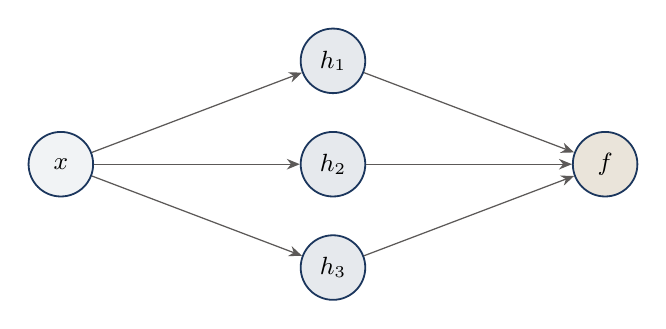
\begin{tikzpicture}[x=1.28cm,y=1.05cm]
  \node[ninput] (x) at (0,0) {$x$};
  \node[nhidden] (h1) at (2.7, 1.25) {$h_1$};
  \node[nhidden] (h2) at (2.7, 0) {$h_2$};
  \node[nhidden] (h3) at (2.7,-1.25) {$h_3$};
  \node[noutput] (y) at (5.4,0) {$f$};
  \draw[nedge] (x) -- (h1);
  \draw[nedge] (x) -- (h2);
  \draw[nedge] (x) -- (h3);
  \draw[nedge] (h1) -- (y);
  \draw[nedge] (h2) -- (y);
  \draw[nedge] (h3) -- (y);
\end{tikzpicture}\\[0.45em]
{\small $h_1=\relu(x)$,\quad $h_2=\relu(x-1)$,\quad $h_3=\relu(x-2)$,\quad $f=h_1-2h_2+h_3$.}
\captionof{figure}{A width-\(3\) realisation of the bump. Every arrow into a hidden unit has weight \(1\); the biases sit inside the formulas for \(h_i\).}
\label{fig:bumpnet}
\end{center}

\solutionpart{b}

Write \(A=\{(1,0),(0,1)\}\) and \(B=\{(0,0),(1,1)\}\). Suppose there exist \(w\in\R^2\) and \(b\in\R\) with \(w^\T x+b>0\) for \(x\in A\) and \(w^\T x+b<0\) for \(x\in B\). Adding the two strict inequalities on \(A\) gives \(w_1+w_2+2b>0\). Adding the two strict inequalities on \(B\) gives \(w_1+w_2+2b<0\). The two conclusions cannot hold simultaneously.

The same intersection can be phrased geometrically, and the geometric form also rules out weak separation. The midpoint \(\tfrac12(1,0)+\tfrac12(0,1) = (\tfrac12,\tfrac12)\) lies in \(\operatorname{conv}(A)\). The same point is \(\tfrac12(0,0)+\tfrac12(1,1)\), so it lies in \(\operatorname{conv}(B)\). Any closed half-space is convex. If \(A\) were contained in a closed half-space and \(B\) in the complementary closed half-space, the two convex hulls would lie in disjoint sets. Figure~\ref{fig:xor} is that crossing.

\begin{center}
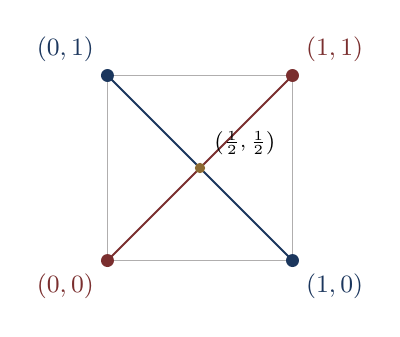
\begin{tikzpicture}[scale=2.35, line cap=round]
  \draw[ink!35, line width=0.4pt] (0,0) rectangle (1,1);
  \draw[accent, line width=0.7pt] (0,0) -- (1,1);
  \draw[navy, line width=0.7pt] (0,1) -- (1,0);
  \fill[accent] (0,0) circle (0.035) node[below left=2pt, font=\small] {$(0,0)$};
  \fill[accent] (1,1) circle (0.035) node[above right=2pt, font=\small] {$(1,1)$};
  \fill[navy] (1,0) circle (0.035) node[below right=2pt, font=\small] {$(1,0)$};
  \fill[navy] (0,1) circle (0.035) node[above left=2pt, font=\small] {$(0,1)$};
  \fill[rulegold] (0.5,0.5) circle (0.028);
  \node[font=\scriptsize, anchor=south west] at (0.52,0.52) {$\bigl(\tfrac12,\tfrac12\bigr)$};
\end{tikzpicture}
\captionof{figure}{The two classes of XOR. The diagonals meet, so no straight cut puts one class on each side.}
\label{fig:xor}
\end{center}

On the Boolean cube the sum of coordinates is \(0\), \(1\), or \(2\), and XOR equals \(1\) precisely on the middle value. The bump satisfies \(f(0)=0\), \(f(1)=1\), and \(f(2)=0\). Therefore
\[
  \operatorname{XOR}(x_1,x_2) = f(x_1+x_2)
  \qquad\text{for all } x\in\{0,1\}^2.
\]
For every such sum one has \(x_1+x_2\le 2\), so the last term of \eqref{eq:bump-relu} is zero. Two hidden units remain:
\begin{equation}
  \operatorname{XOR}(x_1,x_2)
  =
  \relu(x_1+x_2) - 2\,\relu(x_1+x_2-1).
  \label{eq:xor-net}
\end{equation}
The four evaluations are
\begin{center}
\begin{tabular}{@{}cccc@{}}
\toprule
\((x_1,x_2)\) & \(\relu(x_1+x_2)\) & \(\relu(x_1+x_2-1)\) & output \\
\midrule
\((0,0)\) & \(0\) & \(0\) & \(0\) \\
\((1,0)\) & \(1\) & \(0\) & \(1\) \\
\((0,1)\) & \(1\) & \(0\) & \(1\) \\
\((1,1)\) & \(2\) & \(1\) & \(0\) \\
\bottomrule
\end{tabular}
\end{center}
Figure~\ref{fig:xornet} is the corresponding network. The construction is exact on the four Boolean points. It is not a claim about a linear decision boundary in the plane: the function \eqref{eq:xor-net} is piecewise linear on \(\R^2\), and its positive set is a strip between the lines \(x_1+x_2=0\) and \(x_1+x_2=2\), cut by the kink along \(x_1+x_2=1\).

\begin{center}
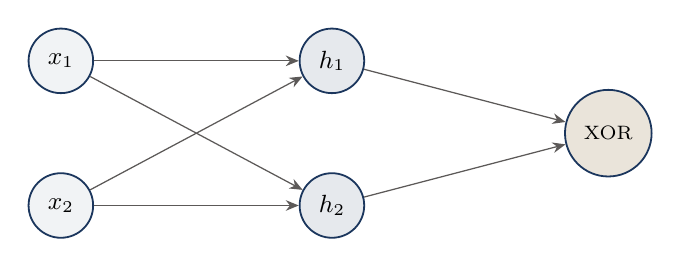
\begin{tikzpicture}[x=1.35cm,y=1.12cm]
  \node[ninput] (x1) at (0, 0.82) {$x_1$};
  \node[ninput] (x2) at (0,-0.82) {$x_2$};
  \node[nhidden] (h1) at (2.55, 0.82) {$h_1$};
  \node[nhidden] (h2) at (2.55,-0.82) {$h_2$};
  \node[noutput, minimum size=11mm] (y) at (5.15,0) {\scriptsize XOR};
  \draw[nedge] (x1) -- (h1);
  \draw[nedge] (x2) -- (h1);
  \draw[nedge] (x1) -- (h2);
  \draw[nedge] (x2) -- (h2);
  \draw[nedge] (h1) -- (y);
  \draw[nedge] (h2) -- (y);
\end{tikzpicture}\\[0.4em]
{\small $h_1=\relu(x_1+x_2)$,\quad $h_2=\relu(x_1+x_2-1)$,\quad $\mathrm{XOR}=h_1-2h_2$.}
\captionof{figure}{Exact ReLU representation of XOR on the Boolean square. Both arrows into a hidden unit carry weight \(1\).}
\label{fig:xornet}
\end{center}

\solutionpart{c}

If \(w_i=0\), the unit \(\relu(w_i x+b_i)\) is constant. If \(w_i\neq 0\), it fails to be differentiable at exactly one point, the kink \(t_i=-b_i/w_i\), where the derivative jumps by \(w_i\). A linear combination of such units, plus a constant, can fail to be differentiable only at the kink locations. Distinct kinks among \(m\) units number at most \(m\), and a cancellation between two jumps at the same location can only remove a breakpoint. Therefore a function of the form \eqref{eq:shallow} has at most \(m\) breakpoints.

The bump has three breakpoints, at \(0\), \(1\), and \(2\), because the slope changes by \(+1\), \(-2\), and \(+1\), none of which is zero. Width \(2\) supplies at most two breakpoints, so no network \eqref{eq:shallow} of width \(2\) equals \(f\) on \(\R\). The width-\(3\) formula \eqref{eq:bump-relu} matches the lower bound and is optimal.

The bound counts breakpoints on the whole line. Agreement merely on a subinterval can only require fewer kinks inside that interval, never more, so the same counting still forbids a width-\(2\) representation of \(f\) on any interval that contains all three slope changes, for instance on \([0,2]\).

\solutionpart{d}

\paragraph{(i).}
On \([0,1]\) the identity coordinate is already a ReLU, because \(\relu(x)=x\). The tent rises with slope \(2\) and then falls with slope \(-2\), so the single interior jump is \(-4\), located at \(1/2\):
\begin{equation}
  s(x) = 2\,\relu(x) - 4\,\relu\bigl(x-\tfrac12\bigr)
  \qquad\text{for all } x\in[0,1].
  \label{eq:tent-relu}
\end{equation}
The check is immediate. On \([0,1/2]\) the second term vanishes and the first equals \(2x\). On \([1/2,1]\),
\[
  2x - 4\bigl(x-\tfrac12\bigr) = 2-2x.
\]
Equivalently, in the shape used for composition below,
\begin{equation}
  s(x)
  =
  \begin{pmatrix} 1 & -1 \end{pmatrix}
  \relu\!\left(
    \begin{pmatrix} 2 \\ 4 \end{pmatrix} x
    +
    \begin{pmatrix} 0 \\ -2 \end{pmatrix}
  \right).
  \label{eq:tent-matrix}
\end{equation}
Indeed \(\relu(2x)-\relu(4x-2)\) reproduces the same two pieces on \([0,1]\). The formula \eqref{eq:tent-matrix} is not obliged to equal the zero extension of \(s\) outside \([0,1]\); the exercise only evaluates it on that interval. For \(x>1\) the expression \(2-2x\) becomes negative, which will matter only if a later composition leaves \([0,1]\). Part~(ii) shows that the iterates we need never do.

\paragraph{(ii).}
The claim is: for every integer \(n\ge 1\) and every integer \(k\) with \(0\le k\le 2^n\),
\[
  s^{\circ n}\!\left(\frac{k}{2^n}\right)
  =
  \begin{cases}
    0 & \text{if \(k\) is even},\\
    1 & \text{if \(k\) is odd},
  \end{cases}
\]
and on each interval \(I_{n,k}=[k/2^n,(k+1)/2^n]\) with \(0\le k<2^n\) the iterate is affine of slope \((-1)^k 2^n\).

For \(n=1\) the claim is the definition of \(s\). Fix \(n\ge 1\) and assume the claim at level \(n\). Nodes and intervals of level \(n+1\) are split at \(1/2\).

\emph{Left half.} If \(0\le k\le 2^n\), the node \(k/2^{n+1}\) lies in \([0,1/2]\) and \(s(k/2^{n+1}) = k/2^n\). The induction hypothesis reads that coarser node by the same index \(k\), so the value is \(0\) or \(1\) according to the parity of \(k\). That is the value required of \(s^{\circ(n+1)}\). Separately, for each interval index \(0\le k<2^n\), the branch \(s(x)=2x\) carries \(I_{n+1,k}\) onto \(I_{n,k}\). The composition with \(s^{\circ n}\) on that image is affine, of slope
\[
  2\cdot(-1)^k\,2^n = (-1)^k\,2^{n+1}.
\]

\emph{Right half.} If \(k=2^n+j\) with \(0\le j\le 2^n\), then
\[
  s\!\left(\frac{2^n+j}{2^{n+1}}\right)
  =
  2-\frac{2^n+j}{2^n}
  =
  \frac{2^n-j}{2^n}.
\]
The index \(2^n-j\) has the same parity as \(j\), and \(k=2^n+j\) has that same parity because \(2^n\) is even. The induction hypothesis therefore returns the value required at the node. For the intervals, take \(0\le j<2^n\). The branch \(s(x)=2-2x\) has slope \(-2\) and maps \(I_{n+1,\,2^n+j}\) onto \(I_{n,\,2^n-j-1}\). That image carries slope \((-1)^{2^n-j-1}2^n = (-1)^{j+1}2^n\), so the composite slope is
\[
  (-2)\cdot(-1)^{j+1}2^n = (-1)^j\,2^{n+1} = (-1)^k\,2^{n+1}.
\]

Both descriptions agree at the shared node \(x=1/2\), where \(s^{\circ(n+1)}(1/2)=0\). Adjacent pieces have opposite nonzero slopes, so they do not merge, and there are exactly \(2^n\) linear pieces. Each piece runs from \(0\) to \(1\) or from \(1\) to \(0\), so the image of \(s^{\circ n}\) is \([0,1]\). In particular every iterate stays inside the interval on which \(s\) was defined.

\paragraph{(iii).}
The deep network uses the factorisation suggested by \eqref{eq:tent-matrix}. Set
\[
  w = \begin{pmatrix} 2 \\ 4 \end{pmatrix},
  \qquad
  b = \begin{pmatrix} 0 \\ -2 \end{pmatrix},
  \qquad
  v = \begin{pmatrix} 1 \\ -1 \end{pmatrix},
  \qquad
  W = w v^\T
  =
  \begin{pmatrix} 2 & -2 \\ 4 & -4 \end{pmatrix}.
\]
The first hidden layer and the readout of a single tent are \(h^{(1)} = \relu(wx+b)\) and \(v^\T h^{(1)}\). For each subsequent hidden layer,
\begin{equation}
  h^{(\ell)} = \relu\!\bigl(W h^{(\ell-1)} + b\bigr),
  \qquad \ell = 2,\ldots,n,
  \label{eq:deep-layer}
\end{equation}
and the network output is \(v^\T h^{(n)}\). Figure~\ref{fig:deep} shows the pattern for \(n=2\); further iterates repeat the same \(2\times 2\) block.

\begin{center}
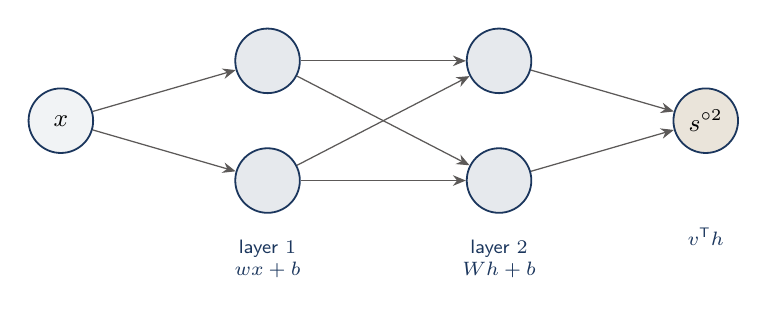
\begin{tikzpicture}[x=1.05cm,y=0.95cm]
  \node[ninput] (x) at (0,0) {$x$};
  \node[nhidden] (a1) at (2.5, 0.8) {};
  \node[nhidden] (a2) at (2.5,-0.8) {};
  \node[nhidden] (b1) at (5.3, 0.8) {};
  \node[nhidden] (b2) at (5.3,-0.8) {};
  \node[noutput] (y) at (7.8,0) {$s^{\circ 2}$};
  \draw[nedge] (x) -- (a1);
  \draw[nedge] (x) -- (a2);
  \draw[nedge] (a1) -- (b1);
  \draw[nedge] (a1) -- (b2);
  \draw[nedge] (a2) -- (b1);
  \draw[nedge] (a2) -- (b2);
  \draw[nedge] (b1) -- (y);
  \draw[nedge] (b2) -- (y);
  \node[ntag, align=center] at (2.5,-1.85) {layer \(1\)\\ $w x+b$};
  \node[ntag, align=center] at (5.3,-1.85) {layer \(2\)\\ $W h+b$};
  \node[ntag] at (7.8,-1.55) {$v^\T h$};
\end{tikzpicture}
\captionof{figure}{Two hidden layers of width \(2\) compute \(s^{\circ 2}\). The first affine map is \(x\mapsto wx+b\); every later hidden map is \(h\mapsto Wh+b\) with \(W=wv^\T\).}
\label{fig:deep}
\end{center}

The proof that the output equals \(s^{\circ n}(x)\) for every \(x\in[0,1]\) is an induction on the number of hidden layers. The case \(n=1\) is \eqref{eq:tent-matrix}. If \(v^\T h^{(\ell-1)} = s^{\circ(\ell-1)}(x)\), the next preactivation collapses through the outer product:
\[
  W h^{(\ell-1)} + b
  =
  w\bigl(v^\T h^{(\ell-1)}\bigr) + b
  =
  w\, s^{\circ(\ell-1)}(x) + b.
\]
Applying \(\relu\) and the readout \(v^\T\) is exactly one evaluation of \eqref{eq:tent-matrix}. Part~(ii) guarantees that the scalar \(s^{\circ(\ell-1)}(x)\) still lies in \([0,1]\), which is the interval on which that evaluation equals the tent. The induction step follows. The network has \(n\) hidden layers, each of width \(2\).

An explicit shallow formula of width \(2^n\) is the kink expansion of part~(a), restricted to \([0,1]\), where \(\relu(x)=x\):
\begin{equation}
  g_n(x)
  =
  2^n \relu(x)
  + \sum_{k=1}^{2^n-1} (-1)^k\, 2^{n+1}\,
    \relu\!\left(x-\frac{k}{2^n}\right).
  \label{eq:shallow-iter}
\end{equation}
There are \(1+(2^n-1)=2^n\) hidden units. On the interval where \(k/2^n < x < (k+1)/2^n\), the derivative is
\[
  g_n'(x)
  =
  2^n + 2^{n+1}\sum_{j=1}^{k}(-1)^j.
\]
The alternating sum equals \(0\) when \(k\) is even and equals \(-1\) when \(k\) is odd, so the derivative equals \(+2^n\) or \(-2^n\) accordingly. This is the slope list of part~(ii). Also \(g_n(0)=0=s^{\circ n}(0)\). Two continuous piecewise-linear functions with the same slopes on the same partition and the same value at \(0\) coincide on \([0,1]\).

The parameter counts are of different orders. The deep network has \(2\) weights and \(2\) biases in the first layer, \(4\) weights and \(2\) biases in each of the other \(n-1\) hidden layers, and \(2\) readout weights, hence \(6n\) parameters. The shallow network has width \(2^n\).

\paragraph{(iv).}
Let \(f_n = s^{\circ n}\) and let \(t_k = k/2^n\). Suppose \(g\) is continuous and piecewise linear on \([0,1]\), with \(M\) linear pieces, and suppose toward a contradiction that \(\norm{f_n-g}_\infty < 1/2\). Then \(g(t_k)<1/2\) for even \(k\) and \(g(t_k)>1/2\) for odd \(k\). By the intermediate-value theorem, each open interval \((t_k,t_{k+1})\) contains a point \(c_k\) with \(g(c_k)=1/2\). These \(2^n\) roots lie in disjoint intervals.

Consider one linear piece of \(g\), defined on a subinterval \(J\). If the piece is not identically equal to \(1/2\), the equation \(g(x)=1/2\) has at most one root in \(J\). If the piece is identically \(1/2\), it still cannot contain two of the points \(c_k\): between \(c_k\) and \(c_{k+1}\) lies the sample \(t_{k+1}\), which would then satisfy \(g(t_{k+1})=1/2\), contradicting the strict inequalities at the samples. Each piece therefore contains at most one \(c_k\). Hence \(M\ge 2^n\).

Equivalently, if \(M\le 2^n-1\), the assumption \(\norm{f_n-g}_\infty<1/2\) is false, so the uniform error is at least \(1/2\).

A one-hidden-layer network of width \(m\) has at most \(m\) breakpoints on \(\R\) by part~(c), hence at most \(m+1\) linear pieces on \([0,1]\). If \(m\le 2^n-2\), then \(m+1\le 2^n-1\), and the uniform error on \(f_n\) is at least \(1/2\). The deep network of paragraph~(iii) equals \(f_n\) exactly, so its uniform error is \(0\).

For \(n=2\) the contrast is especially direct. A shallow network of width \(2^2-2=2\) has error at least \(1/2\). A network of the same width \(2\), with two hidden layers, represents \(s^{\circ 2}\) exactly. Extra width is not a substitute for the second layer at this accuracy. The breakpoint count of part~(c) gives the companion exact-representation bound: \(f_n\) has \(2^n-1\) interior slope changes on \((0,1)\), so any one-hidden-layer representation that is exact on \([0,1]\) needs width at least \(2^n-1\). The explicit network \eqref{eq:shallow-iter} has width \(2^n\), one unit above that lower bound.

\begin{remark}
The piece-count lower bound is not always attained by a ReLU network of that width, because one hidden unit produces a slope change from a one-sided zero derivative, not an arbitrary pair of slopes. For \(n=1\), \(s\) itself is not monotone, whereas every width-\(1\) network \(c+v\relu(wx+b)\) is monotone, so the exact representation of the tent needs width \(2\), matching \eqref{eq:tent-relu}, even though \(s\) has only one interior breakpoint. The exponential statements above do not depend on closing this gap of one unit.
\end{remark}

\solutionpart{e}

Let \(F:[a,b]\to\R\) be continuous and let \(\varepsilon>0\). Uniform continuity provides \(\delta>0\) such that \(\abs{x-x'}<\delta\) implies \(\abs{F(x)-F(x')}<\varepsilon\). Choose a partition \(a=t_0<\cdots<t_m=b\) of mesh less than \(\delta\), and let \(p\) be the piecewise-linear interpolant of \(F\) at the nodes \(t_j\). On each subinterval the interpolant lies between the endpoint values of \(F\), so \(\abs{F-p}<\varepsilon\) throughout \([a,b]\).

It remains only to realise \(p\) by a ReLU network on \([a,b]\). Let \(s_j\) be the slope of \(p\) on \((t_j,t_{j+1})\), and set \(s_{-1}\) formally aside: the formula of part~(a), transplanted to a compact interval, reads
\[
  p(x)
  =
  p(a) + s_0\,\relu(x-a)
  + \sum_{j=1}^{m-1} (s_j-s_{j-1})\,\relu(x-t_j)
  \qquad\text{for } x\in[a,b].
\]
The identity term is a ReLU because \(x-a\ge 0\) on the interval, and \(\relu(x-b)\) is identically zero there, so no unit is required for a right-end correction. This is a network of width at most \(m\), and it equals \(p\), hence it approximates \(F\) within \(\varepsilon\). Density follows. The proof is constructive: the breakpoints are a uniform partition, and the output weights are the slope jumps of the interpolant.

Now suppose the activation \(\rho\) is a polynomial of degree \(d\ge 0\). An affine image of a polynomial is a polynomial of degree at most \(d\), and a coordinatewise application of \(\rho\) multiplies degrees by at most \(d\). After \(L\) hidden layers, every coordinate is a polynomial in the scalar input of degree at most \(d^L\), and the linear readout preserves that bound. Every network in the class therefore represents a member of the vector space \(P_D\) of polynomials of degree at most \(D=d^L\), a space of dimension \(D+1\).

This space is not dense in \(C([0,1])\). Concretely, let \(n=D+1\) and suppose \(q\) is a monic polynomial of degree \(n\), so \(q(x)=x^n-p(x)\) for some \(p\in P_D\). The forward difference of step \(h>0\),
\[
  \Delta_h q(x) = q(x+h)-q(x),
  \qquad
  \Delta_h^{n} = \Delta_h\circ\cdots\circ\Delta_h,
\]
annihilates every polynomial of degree less than \(n\) and satisfies \(\Delta_h^{n}(x^n) = n!\, h^n\). If \(\abs{q}\le\varepsilon\) on \([0,1]\) and \(nh\le 1\), the values of \(q\) that enter \(\Delta_h^{n} q(0)\) lie in \([0,1]\), and
\[
  \abs{\Delta_h^{n} q(0)}
  \le
  \sum_{k=0}^{n}\binom{n}{k}\varepsilon
  =
  2^n\varepsilon.
\]
The left side equals \(n!\, h^n\). Taking \(h=1/n\) yields
\[
  \varepsilon \ge \frac{n!}{(2n)^n} > 0.
\]
Thus no polynomial of degree at most \(D\) can approximate \(x\mapsto x^{D+1}\) more closely than this positive constant, uniformly on \([0,1]\). Polynomial activations, at any finite depth and any finite width, are not universal approximators.

There is no conflict with part~(d). Density says that for each single continuous target and each positive tolerance, some finite width suffices. It does not bound that width uniformly over a class of targets. The functions \(s^{\circ n}\) are uniformly bounded by \(1\), but any shallow network that drives the error below \(1/2\) must have width at least \(2^n-1\), which diverges as the target oscillates. Universal approximation is an existence statement about one fixed function. The depth separation is a statement about how that existence scales with a complexity parameter of the target.

The one-dimensional ReLU argument above does not extend verbatim to several variables, because not every continuous piecewise-linear function of several variables is a shallow ReLU network of width equal to its number of pieces, and uniform approximation by such functions needs a different construction. The general fact is the following.

\begin{proposition}[Leshno, Lin, Pinkus, and Schocken, 1993]
Let \(K\subset\R^d\) be compact and let \(\rho:\R\to\R\) be continuous and not a polynomial. Finite sums
\[
  x \mapsto c + \sum_{i=1}^{m} v_i\,\rho(w_i^\T x + b_i)
\]
are dense in \(C(K)\) for the supremum norm.
\end{proposition}

ReLU meets the hypothesis. Earlier theorems of Cybenko and of Hornik give the same conclusion for continuous sigmoidal activations; those hypotheses exclude ReLU, which is unbounded. Multivariate counts of linear regions, which grow exponentially with depth, are developed by Mont\'ufar, Pascanu, Cho, and Bengio and by Telgarsky. The exponential separation proved in part~(d) is univariate and does not rely on those results.

\begin{thebibliography}{9}
\bibitem{cybenko1989}
G.~Cybenko.
\newblock Approximation by superpositions of a sigmoidal function.
\newblock \emph{Mathematics of Control, Signals, and Systems}, 2:303--314, 1989.

\bibitem{hornik1991}
K.~Hornik.
\newblock Approximation capabilities of multilayer feedforward networks.
\newblock \emph{Neural Networks}, 4(2):251--257, 1991.

\bibitem{leshno1993}
M.~Leshno, V.~Ya.~Lin, A.~Pinkus, and S.~Schocken.
\newblock Multilayer feedforward networks with a nonpolynomial activation function can approximate any function.
\newblock \emph{Neural Networks}, 6(6):861--867, 1993.

\bibitem{montufar2014}
G.~Mont\'ufar, R.~Pascanu, K.~Cho, and Y.~Bengio.
\newblock On the number of linear regions of deep neural networks.
\newblock In \emph{Advances in Neural Information Processing Systems}, 2014.

\bibitem{telgarsky2016}
M.~Telgarsky.
\newblock Benefits of depth in neural networks.
\newblock In \emph{Conference on Learning Theory}, PMLR 49:1517--1539, 2016.
\end{thebibliography}

\end{document}
